% !TEX root = ./pkBeamer.tex
\mode*

\frame{
\mode<presentation>{
\begin{tikzpicture}[remember picture, overlay]
\node[inner sep=0pt,xshift=0cm] at (current page.center){
\tikz \draw[step=2mm,black!50] (0,0) grid (126mm,94mm);
};
{
\node[coordinate] at (1cm,-3.55cm) (start) {};
\node[coordinate] at (1cm,3cm) (end) {};
\node[coordinate] at (10cm,-3.55cm) (endy) {};
\draw[->,thick] (start)--(end);
\draw[->,thick] (start)--(endy);
};
\end{tikzpicture}
}
\frametitle{Bolus: Fixe \enquote{Menge}}



\note<1>{
\begin{itemize}
\item
Zeichnen: 1 Kompartiment, Injektion, dann mit Cylinders.
\item
Konzentration f\"allt in jedem Intervall auf die H\"alfte ab
\item
Zeichenn Abfall �ber Zeit
\end{itemize}
}
\infina
}


\mode<article>{
\vspace{1cm}
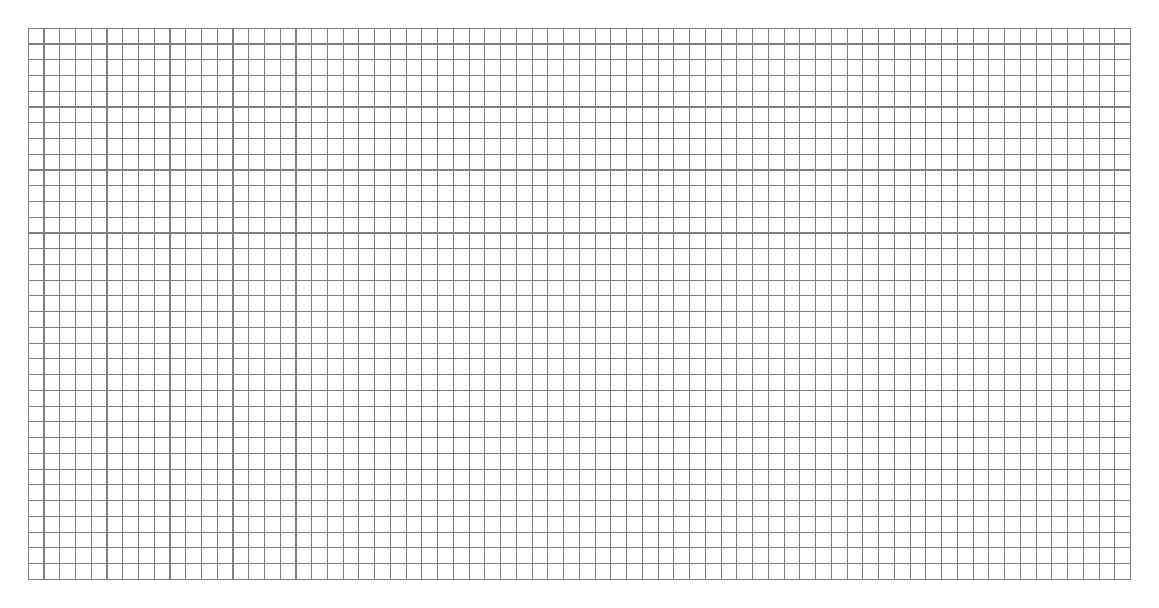
\begin{tikzpicture}[auto]
\node[inner sep=0pt,xshift=0cm] at (current page.center){
\tikz \draw[step=2mm,black!50] (0,0) grid (140mm,70mm);
};
\end{tikzpicture}
}

\mode<article>{\vspace{1cm}
	Unmittelbar nach i.v. Injektion ist die Konzentration im Blut am h�chsten. (theoretisch: $\frac{Dosis}{Blutvolumen}$). Im Gehirn resp. im Gewebe ist aber noch kein Medikament angekommen. Wirkeintritt ist verz�gert gegen�ber Verlauf der Blutkonzentration.

	Konzentration im Blut f�llt exponentiell ab. Geschwindigkeit des Konzentrationsabfalls ist abh�ngig vom Medikament.


}


\frame{
\mode<presentation>{
\begin{tikzpicture}[remember picture, overlay]
\node[inner sep=0pt,xshift=0cm] at (current page.center){
\tikz \draw[step=2mm,black!50] (0,0) grid (126mm,94mm);
};
{
\node[coordinate] at (1cm,-3.55cm) (start) {};
\node[coordinate] at (1cm,3cm) (end) {};
\node[coordinate] at (10cm,-3.55cm) (endy) {};
\draw[->,thick] (start)--(end);
\draw[->,thick] (start)--(endy);
};
\end{tikzpicture}
}

\mode<article>{\newpage}

\frametitle{Konstante Infusion: Konstante (fixe) \enquote{Rate}}
\note<1>{
\begin{itemize}
\item
Zeichnen: Minuten Intervall: Jede Minute wird eine bestimmte Menge verabreicht. 100 mg/min in 10 L
\item
Konzentration w\"urde einfach ansteigen, wenn keine Elimination.
\item
Simulation mit Cylinder 1 Kompartiment (Cl = 0)
\item
Mit Elimination
\item
Auf X-y zeigen wie das passiert. (Behandelt eigentlich schon Elimination)
\end{itemize}
}
\infina
}

\mode<article>{
\vspace{1cm}
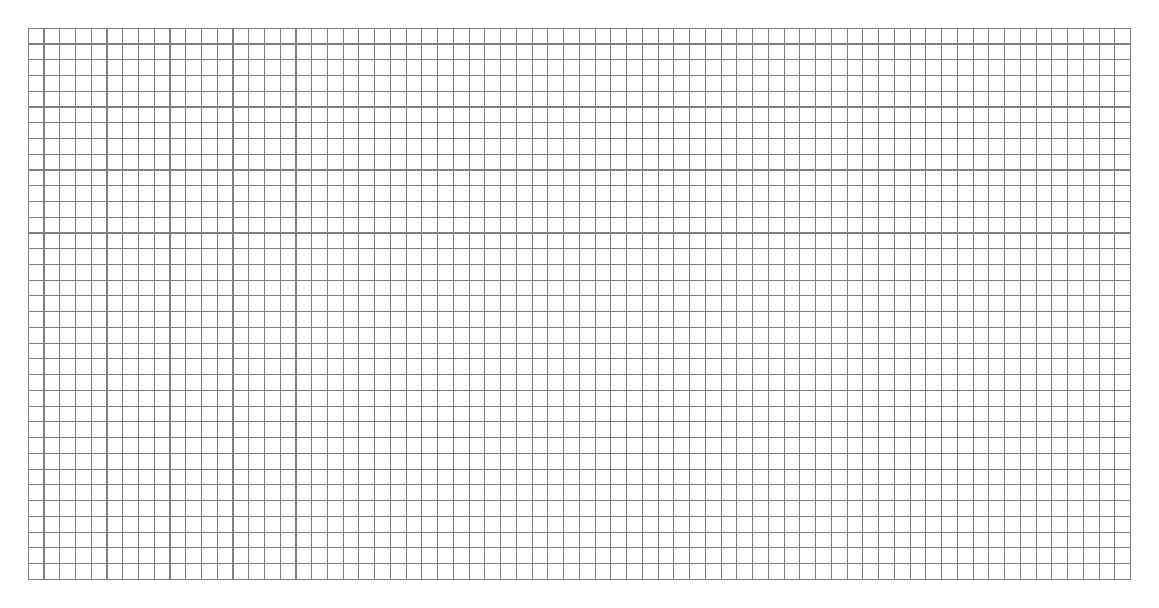
\begin{tikzpicture}[auto]
\node[inner sep=0pt,xshift=0cm] at (current page.center){
\tikz \draw[step=2mm,black!50] (0,0) grid (140mm,70mm);
};
\end{tikzpicture}

\vspace{0.5cm}


Eine konstante Zufuhr(rate) hat nicht einfach eine konstante Konzentration zur Folge. Die Zufuhr muss im Zusammenhang mit der Elimination betrachtet werden (siehe Elimination!) Da die Elimination(srate) proportional zur Konzentration ist, steigt die Konzentration bei konstanter Zufuhr initial an.


Wie lange steigt die Konzentration an?
}





\begin{frame}
\note<1>{
Es ist etwas Komplexer!\\
Kompartimente zeichnen.\\
Zeigen, dass Medi in zentrale Kompartiment verabreicht werden\\
Zeigen der Verteilung\\
Weglassen der Umverteilung\\
Annahme, dass Elimination proportional zu Konzentration.\\
Cylinder: Propofol - IR: Erkl�ren der Dicke der Pfeile = Menge.

}
\end{frame}



